\documentclass{standalone}
%\usepackage{amsmath,amssymb,amsthm,graphicx,epsfig,subfigure,float,url}
\usepackage{amsmath,subfigure,amssymb,amsthm,graphicx,epsfig,float,url}
\usepackage[colorlinks=true]{hyperref}
\usepackage{tikz}
\usepackage{pgf,tikz}
%\usepackage{pdfsync}
%\usepackage{showkeys}
\usepackage{indentfirst}
\usepackage{pgfplots}
\usepackage[applemac]{inputenc}
\usepackage[usenames,dvipsnames]{pstricks}
\newcommand{\R}{\mathbb R}
\begin{document}
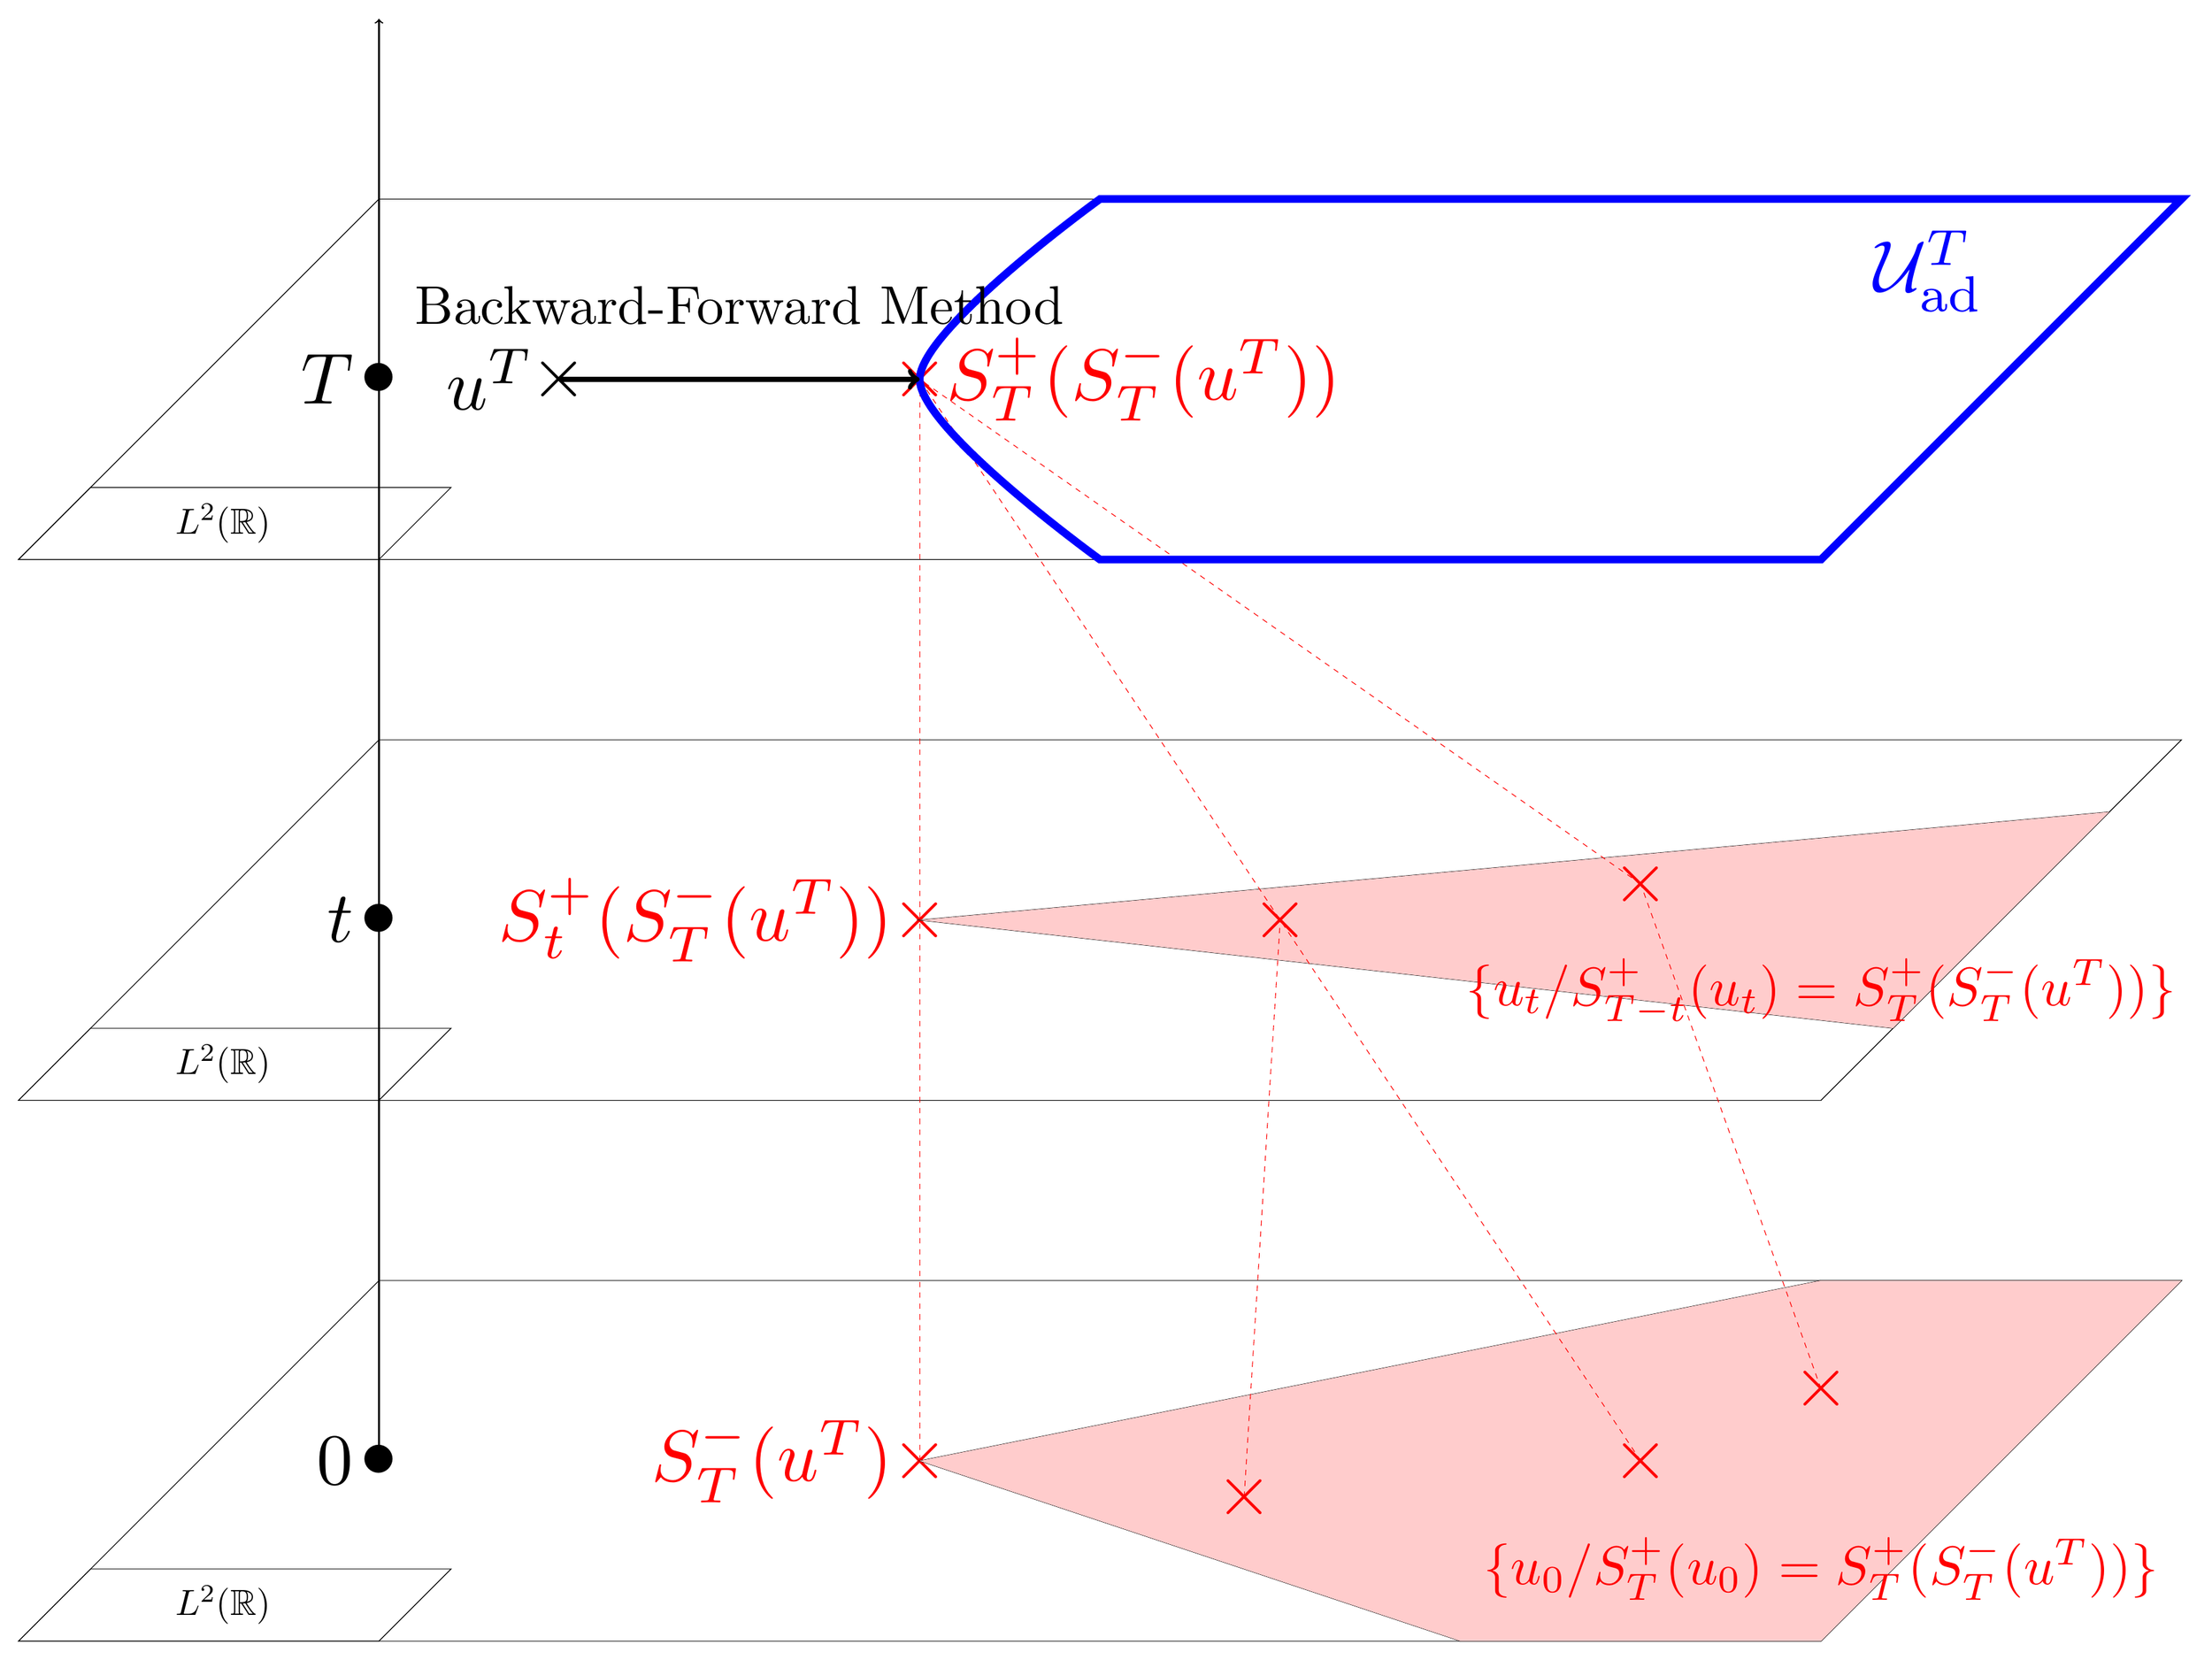
\begin{tikzpicture}[scale=7]
%\fill[color=gray!20] (0,0)--plot [domain=0:1] (\x, {-(1-\x)^2/2+1/2})--(1,0.8)--(0,0.8)--cycle; 
%\fill[color=red!10] (0.2,.4)--plot [domain=0.435:1] (\x, {-(1-\x)^2/2+1/2})--(0.28,.68)--cycle; 
%\draw[->,color=black] (0,0) -- (1.2,0);
%\draw (1.2,0) node[below] {$x$};

%\draw[thick] [domain=0:1] plot (\x, {-(1-\x)^2/2+1/2});
%\draw (0,0) node[below,scale=0.8] {$\bar x - Tf'(u_L)$};
%\draw (1,0) node[below,scale=0.8] {$\bar x - Tf'(u_R)$};
%\draw[dashed] (1,0)--(1,1/2);
%\draw[dashed] (0,1/2)--(1,1/2);
%\draw (1,0.5) node[right,scale=0.8] {$\varphi(\bar x-Tf'(u_R))$};

%\draw[thick] (0.05,0.3) node[above,scale=1] {$u_{M_n}^{n}$};
%\draw[thick] (0.6,0.6)  node[above,scale=1] {$u_0^{n}$};
%\draw[thick] (0.4,0.2) node[below,color=red,scale=1.2] {$ \gamma_2$};
%\draw[thick] (0.8,0.46) node[below,color=black,scale=1.2] {$\gamma_*$};
%\draw (0,0.8) node[left] {$\varphi(x)$};
%\draw [->] (0,0) -- (0,0.8);
%\draw (0.2,.4) node[color=red,below] {$(X_{i},Y_i)$};

%\draw (0,0)--(0.2,0.7);
%\draw (1,0.5)--(0.2,0.7);



%\draw[dashed,color=red] (0.2,.4)--(0.28,.68);
%\draw[dashed,color=red] (0.2,.4)--(0.435,.34);

%\draw (0.5,0) node[below,color=red] {$X_{i+1}$};
%\draw (0.5,-0.02)--(0.5,0.02);
%\draw[dashed] (0.5,0)--(0.5,0.625);

%\draw (0.5,.45) node[color=red] {$\times$} ;
%\draw (0.5,.50) node[color=red] {$\times$} ;
%\draw (0.5,.55) node[color=red] {$\times$} ;
%\draw (0.5,0.60) node[color=red] {$\times$} ;

%\draw (0.7,0.76) node[color=red] {\textcolor{blue}{$-$}} ; 
%\draw (0.72,0.76) node[scale=0.8,right] {\textcolor{blue}{$\gamma \in \Gamma^n(u_L,u_R,\bar x,T)$}  } ; 

%\draw (0.7,0.70) node[color=red] {$\times$} ; 
%\draw (0.72,0.70) node[scale=0.8,right] {Possible values of $\textcolor{red}{Y_{i+1}}$} ; 

%\draw (0.5,.40) node[color=red] {$\times$} ;

%\draw (0.2,.4) node[color=red] {$\bullet$} ;
%\draw[thick] [blue] plot [smooth] coordinates {(0,0) (0.2,0.6) (0.4,0.4) (0.6,0.6) (1,0.5)};

%\draw[thick,dashed] [red] plot [smooth] coordinates {(0,0) (0.2,0.4) (0.4,0.2) (0.6,0.7) (1,0.5)};


%\draw [domain=0:1,color=black!20] plot (\x, {2*\x*(1-\x)});

%\draw[color=blue] (0,0)--(0.1,0.25)--(0.2,.4)--(0.5,.55)--(0.7,0.5)--(0.74,0.54)--(1,0.5);

%\draw [domain=0:0.8] plot (\x, 2*\x*(0.8-\x);
%\draw [domain=0:1] plot (\x, 0.3*\x-0.3*0.35+0.265);
%\draw [->,domain=0:1.2] plot (\x, -0.3*\x);
%\draw[densely dashed] (0,0.36)--(0.41,0.36);
%\draw (0,0.36) node[left] {$F_{\max}(V_b)$};
%\draw (0,0.15) node[left,scale=0.9] {$F_{\alpha}(V_b):=\alpha F_{\max}(V_b)$};

%\draw[densely dashed] (0,0.15)--(1,0.15);
\draw (0,0)--(1,1)--(6,1)--(5,0)--cycle;

\draw (0,1.5)--(1,2.5)--(6,2.5)--(5,1.5)--cycle;

\draw (0,3)--(1,4)--(6,4)--(5,3)--cycle;

\draw[->,thick] (1,0.5)--(1,4.5);
\draw (1,3.5) node[scale=4,left]{$T$};
\draw (1,2) node[scale=4,left]{$t$};
\draw (1,0.5) node[scale=4,left]{$0$};
\draw[color=red!20]  (1,0.5) node[scale=4,color=black,thick]{$\bullet$};
\draw[color=red!20]  (1,3.5) node[scale=4,color=black,thick]{$\bullet$};
\draw[color=red!20]  (1,2) node[scale=4,color=black,thick]{$\bullet$};

\draw  (2.5,0.5) node[scale=4,color=red,thick]{$\times$};
\draw (2.5,0.5) node[scale=4,color=red,thick,left]{$S_T^- (u^T)$};



\draw (2.5,3.5) node[scale=4,color=red,thick]{$\times$};
\draw (2.5,3.5) node[scale=4,color=red,thick,right]{$S_T^+(S_T^- (u^T))$};

\draw (2.5,2) node[scale=4,color=red,thick]{$\times$};
\draw (2.5,2) node[scale=4,color=red,thick,left]{$S_t^+(S_T^- (u^T))$};

\draw  (2.5,0.5)--(5,1)--(6,1)--(5,0)--(4,0)--cycle;
\fill[color=red!20] (2.5,0.5)--(5,1)--(6,1)--(5,0)--(4,0)--cycle;

\draw  (2.5,2)--(5.8,2.3)--(5.2,1.7)--cycle;
\fill[color=red!20] (2.5,2)--(5.8,2.3)--(5.2,1.7)--cycle;

\draw (0.4,0.1) node[scale=2,right] {$L^2(\R)$};
\draw (0,0)--(0.2,0.2)--(1.2,0.2)--(1,0)--cycle;

\draw (0.4,1.6) node[scale=2,right] {$L^2(\R)$};
\draw (0,1.5)--(0.2,1.7)--(1.2,1.7)--(1,1.5)--cycle;

\draw (0.4,3.1) node[scale=2,right] { $L^2(\R)$};
\draw (0,3)--(0.2,3.2)--(1.2,3.2)--(1,3)--cycle;

\draw[color=red,dashed] (2.5,0.5)--(2.5,3.5);
\draw[color=red,dashed] (4.5,0.5)--(2.5,3.5);

\draw[color=red,dashed] (5,0.7)--(4.5,2.1);
\draw  (5,0.7) node[scale=4,color=red] {$\times$};
\draw[color=red,dashed] (4.5,2.1)--(2.5,3.5);
\draw  (4.5,2.1) node[scale=4,color=red] {$\times$};


\draw(5,0.2) node[scale=3,color=red]{$\{u_0 \slash S^+_T(u_0)=S_T^+(S_T^- (u^T))\}$};
\draw(5,1.8) node[scale=3,color=red]{$\{u_t \slash S^+_{T-t}(u_t)=S_T^+(S_T^- (u^T))\}$};

%\draw(4.9,3.9) node[scale=3,color=blue]{$\{S^+_T(u_0)\slash u_0\in  BV(\R)\}$}; 
\draw(5.3,3.8) node[scale=4,color=blue]{$\mathcal{U}_{\text{ad}}^T$}; 
\draw[color=red,dashed]  (3.4,0.4)--(3.5,2);
\draw (3.4,0.4) node[scale=4,color=red] {$\times$};

\draw (3.5,2) node[scale=4,color=red] {$\times$};
\draw (4.5,0.5) node[scale=4,color=red] {$\times$};
%\draw[thick] [blue] plot [smooth] coordinates {(3,3) (2.5,3.5) (3,4) };



\draw[color=blue,line width=1.5mm] plot [smooth] coordinates {(3,3) (2.5,3.5) (3,4)}--(6,4)--(5,3)--cycle;
%\draw[color=blue,thick](2.75,3.2)--(5.2,3.2);
%\draw[color=blue,thick](2.5,3.5)--(5.5,3.5);
%\draw[color=blue,thick](2.75,3.8)--(5.8,3.8);



\draw (1.5,3.5) node[scale=4,left] {$u^T$};
\draw (1.5,3.5) node[scale=4] {$\times$};
\draw (2,3.6) node[above,scale=3]{Backward-Forward \ \\
 Method};


%\draw (2,3.7) node[above,scale=3,color=red]{Reconstruction};
\draw[->,line width=1mm] (1.5,3.5)--(2.5,3.5);
%\draw [->,red] (2,4) to [out=45,in=0] (2,3.5);
%\draw[dashed] (0.1011572875,0)--(0.1011572875,0.1504314574);
%\draw (0.1011572875,0) node[below] {$\check{\rho}_{\alpha}$};
%\draw[dashed] (0.7528427125,0)--(0.7528427125,0.1505685424);
%\draw (0.7528427125,0) node[below] {$\hat{\rho}_{\alpha}$};
%\draw[dashed] (0.8488427125,0)--(0.8488427125,0.2605685424);
%\draw (0.8458427125,-0.01) node[below] {$\rho^*$};
%\draw (0.8488427125,0) node{$\bullet$};
%\draw[dashed] (0.9,0)--(0.9,0.18);
%\draw (0.9,0) node[below] {$\rho^*$};
%\draw (0,0.24) node[left,scale=0.9] {$F_{\alpha}(V_d)$};
%\draw (1,0.47) node[left,scale=0.9] {$F_{\alpha}(V_d)+V_d \rho$};
%\draw (1,0.23) node[left,scale=0.9] {$V_d \rho$};
%\draw (1,0) node[below] {$\rho_{\max}$};
%\draw (0.8,0) node[below] {$\alpha$};
%\draw (0,1/2) node[left] {$f(\rho)-V_b\rho$};
\end{tikzpicture}

\end{document}
